\section{Metric Entropy (Ch. 5)}

\subsection{Covering and Packing}
\begin{definition}[Covering number]
A $\delta$-cover of a set $\mathbb{T}$ with a metric $\rho$ is a set $\{ \theta^1, \cdots, \theta^N \} \subset \mathbb{T} $, such that $\forall \theta \in \mathbb{T}, \exists i \in [N], \rho(\theta, \theta^i) \leq \delta$.
The covering number $N(\delta; \mathbb{T})$ is the cardinality of the smallest $\delta$-cover.
\end{definition}

\begin{definition}[Packing number]
A $\delta$-cover of a set $\mathbb{T}$ with a metric $\rho$ is a set $\{ \theta^1, \cdots, \theta^N \} \subset \mathbb{T} $, such that $\forall \theta \in \mathbb{T}, \exists i \in [N], \rho(\theta, \theta^i) \leq \delta$.

The covering number $N(\delta; \mathbb{T})$ is the cardinality of the smallest $\delta$-cover.
\end{definition}

Below are some common spaces' complexity.
 \begin{center}
    \centering
    \begin{tabular}{lll}
    \toprule
        Space & Rademacher C. & Gaussian C.\\
        \midrule
        $B_1^d(1)$ & 1 & $\sqrt{2 \log d} \pm o(1)$ \\
        $B_2^d(1)$ & $\sqrt{d}$ & $\sqrt{d} - o(1) $ \\
         $B^d_q(1), q>1$ & -  & $\sqrt{\frac{2}{\pi}} d^{1-1/q}$ $\sim$ $c_q d^{1-1/q}$\\
         \bottomrule
    \end{tabular}
 \end{center}

\subsection{Metric entropy and sub-Gaussian processes}
\begin{definition}[sub-Gaussian processes]
For zero-mean random variables $\{X_\theta, \theta \in \mathbb{T}\}$, we say it is a sub-Gaussian process with metric $\rho_X(\cdot, \cdot)$ on $T$ if 
\begin{align*}
    \mathbb{E}[e^{\lambda (X_\theta - X_{\theta'})}] \leq e^{\frac{\lambda^2 \rho^2_X(\theta, \theta')}{2}}, \quad \forall \lambda \in \R \text{ and } \theta, \theta' \in \mathbb{T}.
\end{align*}
\end{definition}
\textbf{Remark}: It can be shown that $X_\theta - X_{\theta'}$ is a sub-Gaussian RV with parameter $\sigma = \sup_{\theta, \theta'} \rho_X(\theta, \theta')$.

\begin{theorem}[One-step discretization bound] For a zero-mean sub-Gaussian process $\{X_\theta, \theta \in \mathbb{T}\}$ with $\rho(\theta, \theta')$, we have an upper bound for any $\delta \in [0, \sigma]$,
\begin{align*}
     \mathbb{E} \sup_{\theta, \theta' \in \mathbb{T}} X_\theta - X_{\theta'} \leq 2 \mathbb{E} \sup_{\theta, \theta' \in \mathbb{T}\atop \rho(\theta, \theta')\leq \delta} (X_\theta - X_{\theta'}) + 4 \sigma \sqrt{\log N(\delta)},
\end{align*}
where $\sigma = \sup_{\theta, \theta' \in \mathbb{T}} \rho(\theta, \theta')$.
\end{theorem}
\begin{proof}
Let $\{\theta_1, \cdots, \theta_N \}$ be a $\sigma$-cover of $T$. For any $\theta \in \mathbb{T}$, we can find at least one $\theta^*$ in the cover, s.t. $\rho(\theta, \theta^*) \leq \delta$, (the same for $\widetilde{\theta^*}$), and hence,
\begin{align*}
    X_\theta - X_{\widetilde{\theta}} & = {\color{red}X_\theta - X_{\theta^*}} + {\color{blue}X_{\theta^*} - X_{\widetilde{\theta}^*}} + {\color{red} X_{\widetilde{\theta}^*} - X_{\widetilde{\theta}}} \\
    & \leq {\color{red} 2\sup_{\rho(\theta, \theta') \leq \delta} (X_\theta - X_{\theta'})} + {\color{blue} \max_{i, j=1, \cdots, N} |X_{\theta_i} - X_{\theta_j}|}
\end{align*}
Below is a figure to illustrate it.
\begin{center}
\tikzset{every picture/.style={line width=0.75pt}} %set default line width to 0.75pt        
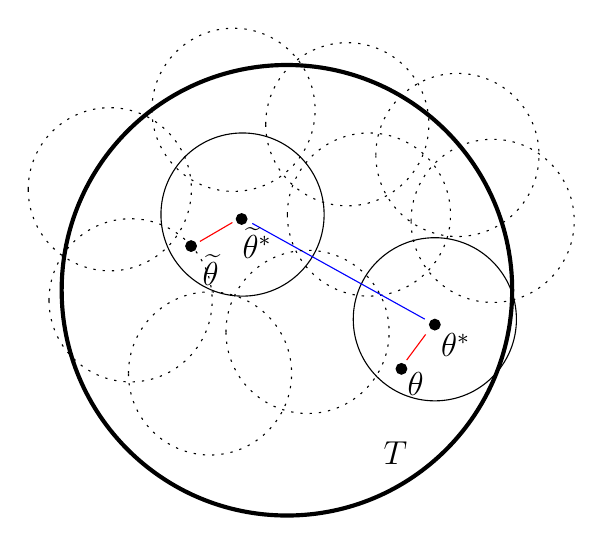
\begin{tikzpicture}[x=0.75pt,y=0.75pt,yscale=-0.87,xscale=0.87]
%uncomment if require: \path (0,365); %set diagram left start at 0, and has height of 365
%Shape: Circle [id:dp20603808590010364] 
\draw  [line width=1.5]  (194.65,169.11) .. controls (194.65,100.21) and (250.5,44.36) .. (319.4,44.36) .. controls (388.29,44.36) and (444.15,100.21) .. (444.15,169.11) .. controls (444.15,238.01) and (388.29,293.86) .. (319.4,293.86) .. controls (250.5,293.86) and (194.65,238.01) .. (194.65,169.11) -- cycle ;
%Shape: Circle [id:dp7264183031125551] 
\draw  [dash pattern={on 0.84pt off 2.51pt}] (176.14,113.18) .. controls (176.14,88.23) and (196.37,68) .. (221.32,68) .. controls (246.27,68) and (266.5,88.23) .. (266.5,113.18) .. controls (266.5,138.13) and (246.27,158.36) .. (221.32,158.36) .. controls (196.37,158.36) and (176.14,138.13) .. (176.14,113.18) -- cycle ;
%Shape: Circle [id:dp5241279298174639] 
\draw   (249.64,127.18) .. controls (249.64,102.23) and (269.87,82) .. (294.82,82) .. controls (319.77,82) and (340,102.23) .. (340,127.18) .. controls (340,152.13) and (319.77,172.36) .. (294.82,172.36) .. controls (269.87,172.36) and (249.64,152.13) .. (249.64,127.18) -- cycle ;
%Shape: Circle [id:dp7096429861126694] 
\draw  [dash pattern={on 0.84pt off 2.51pt}] (244.64,69.18) .. controls (244.64,44.23) and (264.87,24) .. (289.82,24) .. controls (314.77,24) and (335,44.23) .. (335,69.18) .. controls (335,94.13) and (314.77,114.36) .. (289.82,114.36) .. controls (264.87,114.36) and (244.64,94.13) .. (244.64,69.18) -- cycle ;
%Shape: Circle [id:dp9706226409810019] 
\draw  [dash pattern={on 0.84pt off 2.51pt}] (307.64,77.18) .. controls (307.64,52.23) and (327.87,32) .. (352.82,32) .. controls (377.77,32) and (398,52.23) .. (398,77.18) .. controls (398,102.13) and (377.77,122.36) .. (352.82,122.36) .. controls (327.87,122.36) and (307.64,102.13) .. (307.64,77.18) -- cycle ;
%Shape: Circle [id:dp6398302107173852] 
\draw  [dash pattern={on 0.84pt off 2.51pt}] (368.64,94.18) .. controls (368.64,69.23) and (388.87,49) .. (413.82,49) .. controls (438.77,49) and (459,69.23) .. (459,94.18) .. controls (459,119.13) and (438.77,139.36) .. (413.82,139.36) .. controls (388.87,139.36) and (368.64,119.13) .. (368.64,94.18) -- cycle ;
%Shape: Circle [id:dp8128828121822012] 
\draw  [dash pattern={on 0.84pt off 2.51pt}] (319.64,127.18) .. controls (319.64,102.23) and (339.87,82) .. (364.82,82) .. controls (389.77,82) and (410,102.23) .. (410,127.18) .. controls (410,152.13) and (389.77,172.36) .. (364.82,172.36) .. controls (339.87,172.36) and (319.64,152.13) .. (319.64,127.18) -- cycle ;
%Shape: Circle [id:dp05369831229990596] 
\draw  [dash pattern={on 0.84pt off 2.51pt}] (388.14,130.68) .. controls (388.14,105.73) and (408.37,85.5) .. (433.32,85.5) .. controls (458.27,85.5) and (478.5,105.73) .. (478.5,130.68) .. controls (478.5,155.63) and (458.27,175.86) .. (433.32,175.86) .. controls (408.37,175.86) and (388.14,155.63) .. (388.14,130.68) -- cycle ;
%Shape: Circle [id:dp33392831914210697] 
\draw   (356.14,185.18) .. controls (356.14,160.23) and (376.37,140) .. (401.32,140) .. controls (426.27,140) and (446.5,160.23) .. (446.5,185.18) .. controls (446.5,210.13) and (426.27,230.36) .. (401.32,230.36) .. controls (376.37,230.36) and (356.14,210.13) .. (356.14,185.18) -- cycle ;
%Shape: Circle [id:dp7376700951757287] 
\draw  [fill={rgb, 255:red, 0; green, 0; blue, 0 }  ,fill opacity=1 ] (398.36,188.14) .. controls (398.36,186.5) and (399.69,185.18) .. (401.32,185.18) .. controls (402.95,185.18) and (404.28,186.5) .. (404.28,188.14) .. controls (404.28,189.77) and (402.95,191.09) .. (401.32,191.09) .. controls (399.69,191.09) and (398.36,189.77) .. (398.36,188.14) -- cycle ;
%Shape: Circle [id:dp8002681590341161] 
\draw  [fill={rgb, 255:red, 0; green, 0; blue, 0 }  ,fill opacity=1 ] (291.36,129.64) .. controls (291.36,128) and (292.69,126.68) .. (294.32,126.68) .. controls (295.95,126.68) and (297.28,128) .. (297.28,129.64) .. controls (297.28,131.27) and (295.95,132.59) .. (294.32,132.59) .. controls (292.69,132.59) and (291.36,131.27) .. (291.36,129.64) -- cycle ;
%Shape: Circle [id:dp7359208055883519] 
\draw  [fill={rgb, 255:red, 0; green, 0; blue, 0 }  ,fill opacity=1 ] (379.86,212.64) .. controls (379.86,211) and (381.19,209.68) .. (382.82,209.68) .. controls (384.45,209.68) and (385.78,211) .. (385.78,212.64) .. controls (385.78,214.27) and (384.45,215.59) .. (382.82,215.59) .. controls (381.19,215.59) and (379.86,214.27) .. (379.86,212.64) -- cycle ;
%Shape: Circle [id:dp5092748427719243] 
\draw  [fill={rgb, 255:red, 0; green, 0; blue, 0 }  ,fill opacity=1 ] (263.36,144.64) .. controls (263.36,143) and (264.69,141.68) .. (266.32,141.68) .. controls (267.95,141.68) and (269.28,143) .. (269.28,144.64) .. controls (269.28,146.27) and (267.95,147.59) .. (266.32,147.59) .. controls (264.69,147.59) and (263.36,146.27) .. (263.36,144.64) -- cycle ;
%Straight Lines [id:da10457798813301644] 
\draw [color={rgb, 255:red, 255; green, 0; blue, 0 }  ,draw opacity=1 ]   (289.22,131.58) -- (271.22,142.08) ;
%Straight Lines [id:da7764640295404648] 
\draw [color={rgb, 255:red, 0; green, 0; blue, 255 }  ,draw opacity=1 ]   (300.22,132.08) -- (395.72,185.08) ;
%Shape: Circle [id:dp4176329073234546] 
\draw  [dash pattern={on 0.84pt off 2.51pt}] (187.64,174.68) .. controls (187.64,149.73) and (207.87,129.5) .. (232.82,129.5) .. controls (257.77,129.5) and (278,149.73) .. (278,174.68) .. controls (278,199.63) and (257.77,219.86) .. (232.82,219.86) .. controls (207.87,219.86) and (187.64,199.63) .. (187.64,174.68) -- cycle ;
%Shape: Circle [id:dp01245100707397695] 
\draw  [dash pattern={on 0.84pt off 2.51pt}] (285.64,192.18) .. controls (285.64,167.23) and (305.87,147) .. (330.82,147) .. controls (355.77,147) and (376,167.23) .. (376,192.18) .. controls (376,217.13) and (355.77,237.36) .. (330.82,237.36) .. controls (305.87,237.36) and (285.64,217.13) .. (285.64,192.18) -- cycle ;
%Straight Lines [id:da9095478885610673] 
\draw [color={rgb, 255:red, 255; green, 0; blue, 0 }  ,draw opacity=1 ]   (396.22,193.58) -- (385.72,207.75) ;
%Shape: Circle [id:dp5374996882496619] 
\draw  [dash pattern={on 0.84pt off 2.51pt}] (231.64,215.18) .. controls (231.64,190.23) and (251.87,170) .. (276.82,170) .. controls (301.77,170) and (322,190.23) .. (322,215.18) .. controls (322,240.13) and (301.77,260.36) .. (276.82,260.36) .. controls (251.87,260.36) and (231.64,240.13) .. (231.64,215.18) -- cycle ;

% Text Node
\draw (403.32,191.54) node [anchor=north west][inner sep=0.75pt]    {\large$\theta ^{*}$};
% Text Node
\draw (293.36,133.04) node [anchor=north west][inner sep=0.75pt]    {\large$\widetilde{\theta }^{*}$};
% Text Node
\draw (384.82,213.08) node [anchor=north west][inner sep=0.75pt]    {\large$\theta $};
% Text Node
\draw (271.28,148.04) node [anchor=north west][inner sep=0.75pt]    {\large$\widetilde{\theta }$};
% Text Node
\draw (371.5,251.4) node [anchor=north west][inner sep=0.75pt]    {\large$T$};
\end{tikzpicture}
\end{center}
Then, take the expectation on both sides. We use the sub-Gaussian maxima (Thm.~\ref{thm:sub-gaussian-maxima}) on $|X_{\theta_i} - X_{\theta_j}|$, which has  parameter at most $\rho(\theta_i, \theta_j) \leq \sigma$.
Therefore,
\begin{align*}
    \mathbb{E} \sup_{\theta, \theta' \in \mathbb{T}} X_\theta - X_{\theta'} \leq 2 \mathbb{E} \sup_{\theta, \theta' \in \mathbb{T}\atop \rho(\theta, \theta')\leq \delta} (X_\theta - X_{\theta'}) + 4 \sigma \sqrt{\log N(\delta)}
\end{align*}
\end{proof}
\begin{theorem}[One-step discretization bound - corollary] Let $X_\theta = \frac{1}{n} \sum_{i=1}^n \epsilon_i \theta_i$, where $\epsilon$ are Rademacher RVs. Then $\{X_\theta, \theta \in \mathbb{T} \}$ is a sub-Gaussian process with $\rho(\theta, \theta') = \frac{\norm{\theta - \theta'}_2}{\sqrt{n}}$. We have an upper bound as
\begin{align*}
    \mathcal{R}_n(T) \leq \frac{1}{\sqrt{n}} \mathbb{E} \sup_{\theta, \theta' \in \mathbb{T}} X_\theta - X_{\theta'} \leq \frac{2}{\sqrt{n}}[\delta \sqrt{n} + 2\sigma \sqrt{\log N(\delta}],
\end{align*}
\end{theorem}
\textbf{Remark}: This provides a usage of sub-Gaussian process, to bound the Rademacher complexity.

\begin{theorem}[Dudley's integral] 
Let $\{X_\theta, \theta \in \mathbb{T} \}$ be a zero-mean sub-Gaussian process with a  metric $\rho$. Define $D = \sup_{\theta, \theta'} \rho(\theta, \theta')$.
\begin{align*}
    \mathbb{E} \sup_{\theta, \theta'} X_\theta - X_{\theta'} \leq 2 \mathbb{E} \sup_{\rho(\theta, \theta')} X_\theta - X_{\theta'} + 16 \int^D_{\delta/4} \sqrt{\log N(t)} \mathrm{d}t.
\end{align*}
\end{theorem}
\textbf{Remark}: The Dudley's integral (sometimes) achieves a tighter bound on the last term of $4\sigma \sqrt{\log N(\delta)}$ by chaining method.

\begin{center}
\tikzset{every picture/.style={line width=0.75pt}} %set default line width to 0.75pt        

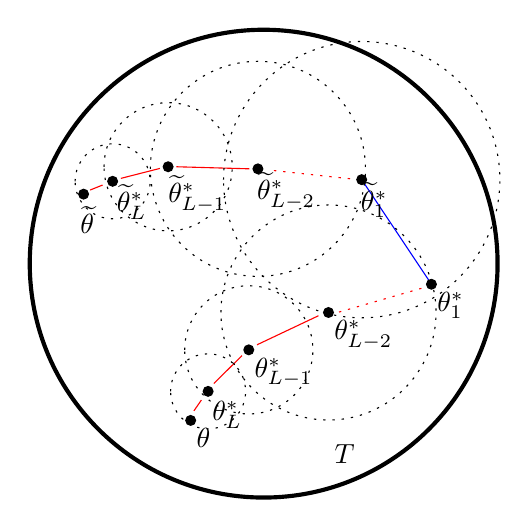
\begin{tikzpicture}[x=0.75pt,y=0.75pt,yscale=-0.8,xscale=0.8]
%uncomment if require: \path (0,365); %set diagram left start at 0, and has height of 365

%Shape: Circle [id:dp19684007366944822] 
\draw  [line width=1.5]  (221.91,172.73) .. controls (221.91,94.93) and (284.98,31.86) .. (362.78,31.86) .. controls (440.58,31.86) and (503.65,94.93) .. (503.65,172.73) .. controls (503.65,250.52) and (440.58,313.59) .. (362.78,313.59) .. controls (284.98,313.59) and (221.91,250.52) .. (221.91,172.73) -- cycle ;
%Shape: Circle [id:dp37546481991304903] 
\draw  [fill={rgb, 255:red, 0; green, 0; blue, 0 }  ,fill opacity=1 ] (326.36,249.64) .. controls (326.36,248) and (327.69,246.68) .. (329.32,246.68) .. controls (330.95,246.68) and (332.28,248) .. (332.28,249.64) .. controls (332.28,251.27) and (330.95,252.59) .. (329.32,252.59) .. controls (327.69,252.59) and (326.36,251.27) .. (326.36,249.64) -- cycle ;
%Shape: Circle [id:dp2963294714242435] 
\draw  [fill={rgb, 255:red, 0; green, 0; blue, 0 }  ,fill opacity=1 ] (268.86,123.14) .. controls (268.86,121.5) and (270.19,120.18) .. (271.82,120.18) .. controls (273.45,120.18) and (274.78,121.5) .. (274.78,123.14) .. controls (274.78,124.77) and (273.45,126.09) .. (271.82,126.09) .. controls (270.19,126.09) and (268.86,124.77) .. (268.86,123.14) -- cycle ;
%Shape: Circle [id:dp5420621191274886] 
\draw  [fill={rgb, 255:red, 0; green, 0; blue, 0 }  ,fill opacity=1 ] (315.86,267.14) .. controls (315.86,265.5) and (317.19,264.18) .. (318.82,264.18) .. controls (320.45,264.18) and (321.78,265.5) .. (321.78,267.14) .. controls (321.78,268.77) and (320.45,270.09) .. (318.82,270.09) .. controls (317.19,270.09) and (315.86,268.77) .. (315.86,267.14) -- cycle ;
%Shape: Circle [id:dp9995668227699503] 
\draw  [fill={rgb, 255:red, 0; green, 0; blue, 0 }  ,fill opacity=1 ] (251.37,130.87) .. controls (251.37,129.24) and (252.69,127.91) .. (254.32,127.91) .. controls (255.96,127.91) and (257.28,129.24) .. (257.28,130.87) .. controls (257.28,132.5) and (255.96,133.83) .. (254.32,133.83) .. controls (252.69,133.83) and (251.37,132.5) .. (251.37,130.87) -- cycle ;
%Straight Lines [id:da6606938671394016] 
\draw [color={rgb, 255:red, 255; green, 0; blue, 0 }  ,draw opacity=1 ]   (265.78,125.37) -- (258.28,128.37) ;
%Straight Lines [id:da31124628774224106] 
\draw [color={rgb, 255:red, 0; green, 0; blue, 255 }  ,draw opacity=1 ]   (421.82,122.14) -- (463.82,185.14) ;
%Shape: Circle [id:dp6240904030753718] 
\draw  [dash pattern={on 0.84pt off 2.51pt}] (306.73,249.64) .. controls (306.73,237.16) and (316.85,227.05) .. (329.32,227.05) .. controls (341.8,227.05) and (351.91,237.16) .. (351.91,249.64) .. controls (351.91,262.11) and (341.8,272.22) .. (329.32,272.22) .. controls (316.85,272.22) and (306.73,262.11) .. (306.73,249.64) -- cycle ;
%Straight Lines [id:da02663647664030422] 
\draw [color={rgb, 255:red, 255; green, 0; blue, 0 }  ,draw opacity=1 ]   (325.28,254.87) -- (320.78,261.37) ;
%Shape: Circle [id:dp0641440846668293] 
\draw  [fill={rgb, 255:red, 0; green, 0; blue, 0 }  ,fill opacity=1 ] (302.28,114.37) .. controls (302.28,112.74) and (303.6,111.41) .. (305.24,111.41) .. controls (306.87,111.41) and (308.19,112.74) .. (308.19,114.37) .. controls (308.19,116) and (306.87,117.33) .. (305.24,117.33) .. controls (303.6,117.33) and (302.28,116) .. (302.28,114.37) -- cycle ;
%Straight Lines [id:da6203583479569572] 
\draw [color={rgb, 255:red, 255; green, 0; blue, 0 }  ,draw opacity=1 ]   (300.28,115.37) -- (276.78,121.37) ;
%Shape: Circle [id:dp35910966149356827] 
\draw  [fill={rgb, 255:red, 0; green, 0; blue, 0 }  ,fill opacity=1 ] (356.36,115.64) .. controls (356.36,114) and (357.69,112.68) .. (359.32,112.68) .. controls (360.95,112.68) and (362.28,114) .. (362.28,115.64) .. controls (362.28,117.27) and (360.95,118.59) .. (359.32,118.59) .. controls (357.69,118.59) and (356.36,117.27) .. (356.36,115.64) -- cycle ;
%Straight Lines [id:da2672880550331598] 
\draw [color={rgb, 255:red, 255; green, 0; blue, 0 }  ,draw opacity=1 ]   (354.19,115.61) -- (310.19,114.37) ;
%Shape: Circle [id:dp3275093497755006] 
\draw  [fill={rgb, 255:red, 0; green, 0; blue, 0 }  ,fill opacity=1 ] (350.86,224.64) .. controls (350.86,223) and (352.19,221.68) .. (353.82,221.68) .. controls (355.45,221.68) and (356.78,223) .. (356.78,224.64) .. controls (356.78,226.27) and (355.45,227.59) .. (353.82,227.59) .. controls (352.19,227.59) and (350.86,226.27) .. (350.86,224.64) -- cycle ;
%Straight Lines [id:da06735315583419843] 
\draw [color={rgb, 255:red, 255; green, 0; blue, 0 }  ,draw opacity=1 ]   (349.78,228.09) -- (332.78,244.87) ;
%Shape: Circle [id:dp962698819630809] 
\draw  [fill={rgb, 255:red, 0; green, 0; blue, 0 }  ,fill opacity=1 ] (398.86,202.14) .. controls (398.86,200.5) and (400.19,199.18) .. (401.82,199.18) .. controls (403.45,199.18) and (404.78,200.5) .. (404.78,202.14) .. controls (404.78,203.77) and (403.45,205.09) .. (401.82,205.09) .. controls (400.19,205.09) and (398.86,203.77) .. (398.86,202.14) -- cycle ;
%Straight Lines [id:da8264622210983994] 
\draw [color={rgb, 255:red, 255; green, 0; blue, 0 }  ,draw opacity=1 ]   (395.78,204.09) -- (358.78,221.59) ;
%Shape: Circle [id:dp12588135320242566] 
\draw  [fill={rgb, 255:red, 0; green, 0; blue, 0 }  ,fill opacity=1 ] (460.86,185.14) .. controls (460.86,183.5) and (462.19,182.18) .. (463.82,182.18) .. controls (465.45,182.18) and (466.78,183.5) .. (466.78,185.14) .. controls (466.78,186.77) and (465.45,188.09) .. (463.82,188.09) .. controls (462.19,188.09) and (460.86,186.77) .. (460.86,185.14) -- cycle ;
%Shape: Circle [id:dp79173620737152] 
\draw  [fill={rgb, 255:red, 0; green, 0; blue, 0 }  ,fill opacity=1 ] (418.86,122.14) .. controls (418.86,120.5) and (420.19,119.18) .. (421.82,119.18) .. controls (423.45,119.18) and (424.78,120.5) .. (424.78,122.14) .. controls (424.78,123.77) and (423.45,125.09) .. (421.82,125.09) .. controls (420.19,125.09) and (418.86,123.77) .. (418.86,122.14) -- cycle ;
%Straight Lines [id:da1378960949499275] 
\draw [color={rgb, 255:red, 255; green, 0; blue, 0 }  ,draw opacity=1 ] [dash pattern={on 0.84pt off 2.51pt}]  (414.78,121.59) -- (366.19,116.37) ;
%Straight Lines [id:da5506540246280685] 
\draw [color={rgb, 255:red, 255; green, 0; blue, 0 }  ,draw opacity=1 ] [dash pattern={on 0.84pt off 2.51pt}]  (457.78,187.59) -- (408.19,201.87) ;
%Shape: Circle [id:dp2677220432717424] 
\draw  [dash pattern={on 0.84pt off 2.51pt}] (315.22,224.64) .. controls (315.22,203.32) and (332.5,186.04) .. (353.82,186.04) .. controls (375.14,186.04) and (392.42,203.32) .. (392.42,224.64) .. controls (392.42,245.95) and (375.14,263.24) .. (353.82,263.24) .. controls (332.5,263.24) and (315.22,245.95) .. (315.22,224.64) -- cycle ;
%Shape: Circle [id:dp20125267536050773] 
\draw  [dash pattern={on 0.84pt off 2.51pt}] (337.04,202.14) .. controls (337.04,166.36) and (366.04,137.36) .. (401.82,137.36) .. controls (437.6,137.36) and (466.6,166.36) .. (466.6,202.14) .. controls (466.6,237.91) and (437.6,266.91) .. (401.82,266.91) .. controls (366.04,266.91) and (337.04,237.91) .. (337.04,202.14) -- cycle ;
%Shape: Circle [id:dp29151738350801537] 
\draw  [dash pattern={on 0.84pt off 2.51pt}] (249.23,123.14) .. controls (249.23,110.66) and (259.35,100.55) .. (271.82,100.55) .. controls (284.3,100.55) and (294.41,110.66) .. (294.41,123.14) .. controls (294.41,135.61) and (284.3,145.72) .. (271.82,145.72) .. controls (259.35,145.72) and (249.23,135.61) .. (249.23,123.14) -- cycle ;
%Shape: Circle [id:dp9553417291902377] 
\draw  [dash pattern={on 0.84pt off 2.51pt}] (266.64,114.37) .. controls (266.64,93.05) and (283.92,75.77) .. (305.24,75.77) .. controls (326.55,75.77) and (343.84,93.05) .. (343.84,114.37) .. controls (343.84,135.69) and (326.55,152.97) .. (305.24,152.97) .. controls (283.92,152.97) and (266.64,135.69) .. (266.64,114.37) -- cycle ;
%Shape: Circle [id:dp1802524110332464] 
\draw  [dash pattern={on 0.84pt off 2.51pt}] (294.54,115.64) .. controls (294.54,79.86) and (323.54,50.86) .. (359.32,50.86) .. controls (395.1,50.86) and (424.1,79.86) .. (424.1,115.64) .. controls (424.1,151.41) and (395.1,180.41) .. (359.32,180.41) .. controls (323.54,180.41) and (294.54,151.41) .. (294.54,115.64) -- cycle ;
%Shape: Circle [id:dp03052433859047765] 
\draw  [dash pattern={on 0.84pt off 2.51pt}] (338.62,122.14) .. controls (338.62,76.18) and (375.87,38.93) .. (421.82,38.93) .. controls (467.77,38.93) and (505.03,76.18) .. (505.03,122.14) .. controls (505.03,168.09) and (467.77,205.34) .. (421.82,205.34) .. controls (375.87,205.34) and (338.62,168.09) .. (338.62,122.14) -- cycle ;

% Text Node
\draw (330.32,254.04) node [anchor=north west][inner sep=0.75pt]    {$\theta _{L}^{*}$};
% Text Node
\draw (272.82,123.58) node [anchor=north west][inner sep=0.75pt]    {$\widetilde{\theta }_{L}^{*}$};
% Text Node
\draw (320.82,270.54) node [anchor=north west][inner sep=0.75pt]    {$\theta $};
% Text Node
\draw (250.78,136.54) node [anchor=north west][inner sep=0.75pt]    {$\widetilde{\theta }$};
% Text Node
\draw (404,280.4) node [anchor=north west][inner sep=0.75pt]    {$T$};
% Text Node
\draw (303.82,118.04) node [anchor=north west][inner sep=0.75pt]    {$\widetilde{\theta }_{L-1}^{*}$};
% Text Node
\draw (357.32,116.04) node [anchor=north west][inner sep=0.75pt]    {$\widetilde{\theta }_{L-2}^{*}$};
% Text Node
\draw (355.82,228.04) node [anchor=north west][inner sep=0.75pt]    {$\theta _{L-1}^{*}$};
% Text Node
\draw (403.82,205.54) node [anchor=north west][inner sep=0.75pt]    {$\theta _{L-2}^{*}$};
% Text Node
\draw (465.82,188.54) node [anchor=north west][inner sep=0.75pt]    {$\theta _{1}^{*}$};
% Text Node
\draw (419.82,122.54) node [anchor=north west][inner sep=0.75pt]    {$\widetilde{\theta }_{1}^{*}$};


\end{tikzpicture}
\end{center}
\begin{proof}
Define $L = \ceil{\log_2 \frac{D}{\delta} }$ sets of $\delta_i$-covers $\mathcal{C}_i$, where $\delta_i = \frac{1}{2^i}D$. Let $N(\delta_i)$ denote the covering number in $\mathcal{C}_i$.
\begin{align*}
X_{\theta_{L}}-X_{\widetilde{\theta_{L}}} & \leq {\color{red} X_{\theta_L}-X_{\theta^*_{L-1}}} + {\color{blue} X_{\theta^*_{L-1}}-X_{\widetilde{\theta}^*_{L-1}}}+{\color{red}X_{\widetilde{\theta}^{\star}_{L-1}}-X_{\widetilde{\theta_L}}} \\
&= {\color{red} 2 \max _{\theta \in \mathcal{C}_{L}} X_{\theta}-X_{\theta^*_{L-1}}} + {\color{blue}\max_{\theta, \theta^{\prime} \in \mathcal{C}_{L-1}} X_{\theta}-X_{\theta^{\prime}}} \\
& \cdots\cdots \\
& \leq  {\color{red}2 \sum_{i=2}^{L} \max_{\theta \in \mathcal{C}_{i}} X_{\theta}-X_{\theta^*_{i-1}}} + {\color{blue}\max _{\theta, \theta^{\prime} \in \mathcal{C}_{1}} X_{\theta}-X_{\theta^{\prime}}}
\end{align*}
Next, we use sub-Gaussian maxima,
\begin{align*}
    \EE \, {\color{red}\max_{\theta \in \mathcal{C}_{i}} X_{\theta}-X_{\theta^*_{i-1}}} & \leq 2 \delta_{i-1} \sqrt{\log |\mathcal{C}_i|} \leq 2 \cdot \frac{D}{2^{i-1}} \sqrt{\log N\left(\frac{D}{2^{i-1}}\right)} \\
    & \leq 8 \int_{D/2^{i-1}}^{D/2^i} \sqrt{\log N\left(t\right)} \mathrm{d} t
\end{align*}
Putting things together, we get
\begin{align*}
\mathbb{E} \max _{\theta, \tilde{\theta} \in \mathcal{C}_{L}} X_{\theta}-X_{\tilde{\theta}} & \leq 16 \sum_{i=2}^{L}\int_{\frac{D}{2^{i-1}}}^{\frac{D}{2^i}} \sqrt{\log N\left(t\right)} \mathrm{d} t + 2 D \sqrt{\log N\left(\frac{D}{2}\right)} \\
& \leq 16 \int_{\delta / 4}^{D} \sqrt{\log N_{\mathbb{T}}(t)} \mathrm{d} t
\end{align*}
This gives the desired form.
\end{proof}


